\documentclass[
 size=12pt,
 paper=smartboard, %a4paper, smartboard, screen
 mode=present, %present, handout, print
 display=slides, % slidesnotes, notes, slides
 style=tuliplab,  % TULIP Lab style
 pauseslide,
 fleqn,leqno,clock]{powerdot}

\usepackage{amssymb}
\usepackage{amsmath}
\usepackage{rotating}
\usepackage{graphicx}
\usepackage{boxedminipage}
\usepackage{media9}
\usepackage{rotate}
\usepackage{calc}
\usepackage[absolute]{textpos}
\usepackage{psfrag,overpic}
\usepackage{fouriernc}
\usepackage{pstricks,pst-node,pst-text,pst-3d,pst-grad}
\usepackage{moreverb,epsfig,color,subfigure}
\usepackage{color}
\usepackage{pstricks}
\usepackage{pstricks-add}
\usepackage{pst-text}
\usepackage{pst-node, pst-tree}
\usepackage{booktabs}
\usepackage{etex}
\usepackage{breqn}
\usepackage{multirow}
% \usepackage{pst-rel-points}
\usepackage{listings}
\usepackage{hyperref}
\hypersetup{ % TODO: PDF meta Data
  pdftitle={Presentation Title},
  pdfauthor={Gang Li},
  pdfpagemode={FullScreen},
  pdfborder={0 0 0}
}


% \usepackage{auto-pst-pdf}
% package to show source code

\definecolor{LightGray}{rgb}{0.9,0.9,0.9}
\newlength{\pixel}\setlength\pixel{0.000714285714\slidewidth}
\setlength{\TPHorizModule}{\slidewidth}
\setlength{\TPVertModule}{\slideheight}
\newcommand\highlight[1]{\fbox{#1}}
\newcommand\icite[1]{{\footnotesize [#1]}}

\newcommand\twotonebox[2]{\fcolorbox{pdcolor2}{pdcolor2}{#1\vphantom{#2}}\fcolorbox{pdcolor2}{white}{#2\vphantom{#1}}}
\newcommand\twotoneboxo[2]{\fcolorbox{pdcolor2}{pdcolor2}{#1}\fcolorbox{pdcolor2}{white}{#2}}
\newcommand\vpspace[1]{\vphantom{\vspace{#1}}}
\newcommand\hpspace[1]{\hphantom{\hspace{#1}}}
\newcommand\COMMENT[1]{}

\newcommand\placepos[3]{\hbox to\z@{\kern#1
        \raisebox{-#2}[\z@][\z@]{#3}\hss}\ignorespaces}


%%%%%%%%%%%%%%%%%%%%%%%%%%%%%%%%%%%%%%%%%%%%%%%%%%%%%%%%%%%%%%%%%%%%%%%%%%
%%% title
%%% TODO: Customize to your Own Title, Name, Address
%%%
\title{FLIP(01) Final-term Presentation}
\author{Rongxin Xu\\
Hunan University
% \href{mailto:gangli@acm.org}{gangli@acm.org}
% \and % more authors
}
\date{27 February 2020}



% Customize the setting of slides
\pdsetup{
% TODO: Customize the left footer, and right footer
rf={\copyright \emph{FLIP(01)}},
cf={FLIP(01) Presentation },
}


% Starts the document
\begin{document}

\maketitle

%%==========================================================================================
%%
\begin{slide}[toc=,bm=]{Outline}
	\tableofcontents[content=sections]
\end{slide}
%%
%%==========================================================================================

\section{Problem Statement}

\begin{slide}{Problem Description}
	\begin{center}
		\twotonebox{\rotatebox{90}{Defn}}{\parbox{.96\textwidth}
			{
This is a problem with natural language processing.
The ubiquitousness of smartphones enables 
people to announce an emergency they’re 
observing in real-time. So the target is
Predict whether a real disaster has occurred 
based on keywords, location, and twitter text.}}
	\end{center}
\end{slide}

\begin{slide}{Data Set}
	\begin{center}
		\twotonebox{\rotatebox{90}{Defn}}{\parbox{.96\textwidth}
			{There are 3 data sets with a total of 5 attributes,
				the fllowings ~\cref{tbl:Attribute Information} are the	name and meaning of attributes.
			}}
	\end{center}
\begin{description}
	\item[train.csv] the training set.
	\item[test.csv] the test set.
	\item[sample\_submission.csv] a sample submission file in the correct format.
\end{description}

\begin{table}[htbp]
	\label{tbl:Attribute Information}
	\centering
	\caption{Attribute Information}
	\begin{tabular}{llllll}
		\hline
		% after \\: \hline or \cline{col1-col2} \cline{col3-col4} ...
		Attributes & Information                                                                            \\
		\hline
		id   & a unique identifier for each tweet                                                               \\
		text    & the text of the tweet                                                                         \\
		location     & the location the tweet was sent from (may be blank)                                      \\
		keyword     & a particular keyword from the tweet (may be blank)                                        \\
		target    &  in train.csv only, this denotes whether a tweet is about a real disaster (1) or not (0)    \\                                               \\
		\hline
		%\bottomrule
	\end{tabular}
\end{table}
\end{slide}

\section{Exploratory Data Analysis}
%
\begin{slide}{Keyword and Location}
\subsubsection{Missing Values}
Both training and test set have same ratio 
of missing values in keyword and location.
the fllowings ~\cref{fig:missing-values-of-keyword-and-location} are the  
missing values of keyword and location.

\begin{itemize}
	\item
	0.8\% of keyword is missing in both training and test set
	\item
	33\% of location is missing in both training and test set
\end{itemize}


\begin{figure}[tbph]
	\centering
	\includegraphics[scale=0.3]{"Figures/Missing Values of Keyword and Location.pdf"}
	\caption{Missing Values of Keyword and Location}
	\label{fig:missing-values-of-keyword-and-location}
\end{figure}

Since missing value ratios between training and test set 
are too close, they are most probably taken from the 
same sample. Missing values in those features are 
filled with no\_keyword and no\_location respectively.
\end{slide}

\begin{slide}{Data Visualization}
	\begin{center}
		\twotonebox{\rotatebox{90}{Exp}}{\parbox{.96\textwidth}
			{Use EDA to plot the distribution of the data,
				can observate the data intuitively and
				find the relation between the attribute values.
			}}
	\end{center}
	\begin{center}
		\begin{itemize}
			\item Figures
			      \begin{itemize}
				      \item Histogrm
				      \item Boxplot
				      \item Scatterplot Plot
				      \item Correllogram
			      \end{itemize}
		\end{itemize}
	\end{center}
\end{slide}

\begin{slide}{Data Visualization}
	\begin{center}
		\twotonebox{\rotatebox{90}{Exp}}{\parbox{.96\textwidth}
			{It seems that item\_id and
				shop\_id has a huge impact on sales and sales tend to decline
				with the date.
			}}
	\end{center}

	\begin{center}
		\includegraphics[width=.4\linewidth,height=.4\linewidth]{figures/his_1.eps}
	\end{center}
\end{slide}

\begin{slide}{Data Visualization}
	\begin{center}
		\twotonebox{\rotatebox{90}{Exp}}{\parbox{.96\textwidth}
			{When analyzing the data,
				the boxplot can effectively
				help us identify the characteristics of the data:
				visually identify outliers in the dataset or
				determine the data dispersion and
				bias of the data set.
				We can see that the outliers are very small,
				so can be ignored.
			}}
	\end{center}

	\begin{center}
		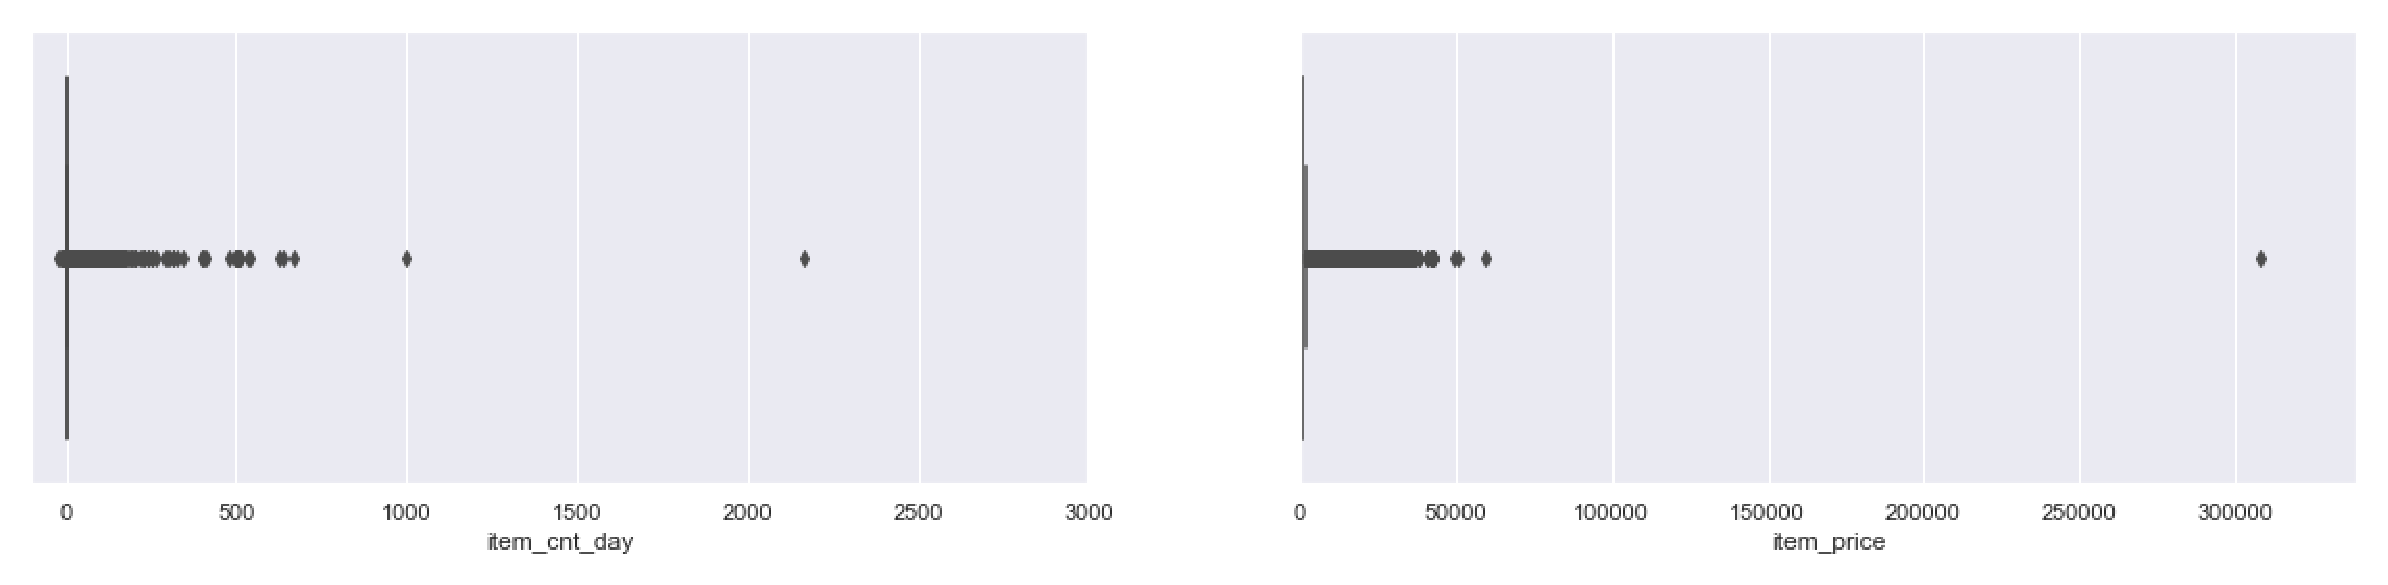
\includegraphics[width=.4\linewidth,height=.4\linewidth]{figures/boxplot.eps}
		\quad\includegraphics[width=.4\linewidth,height=.4\linewidth]{figures/corr.eps}
	\end{center}
\end{slide}

\begin{slide}{Data Visualization}
	\begin{center}
		\twotonebox{\rotatebox{90}{Exp}}{\parbox{.96\textwidth}
			{It can be seen from the scatter plot that the daily sales volume
				of the product is mainly concentrated between 0 and 1, and the
				price of the product can also be concentrated.
			}}
	\end{center}
	\begin{center}
		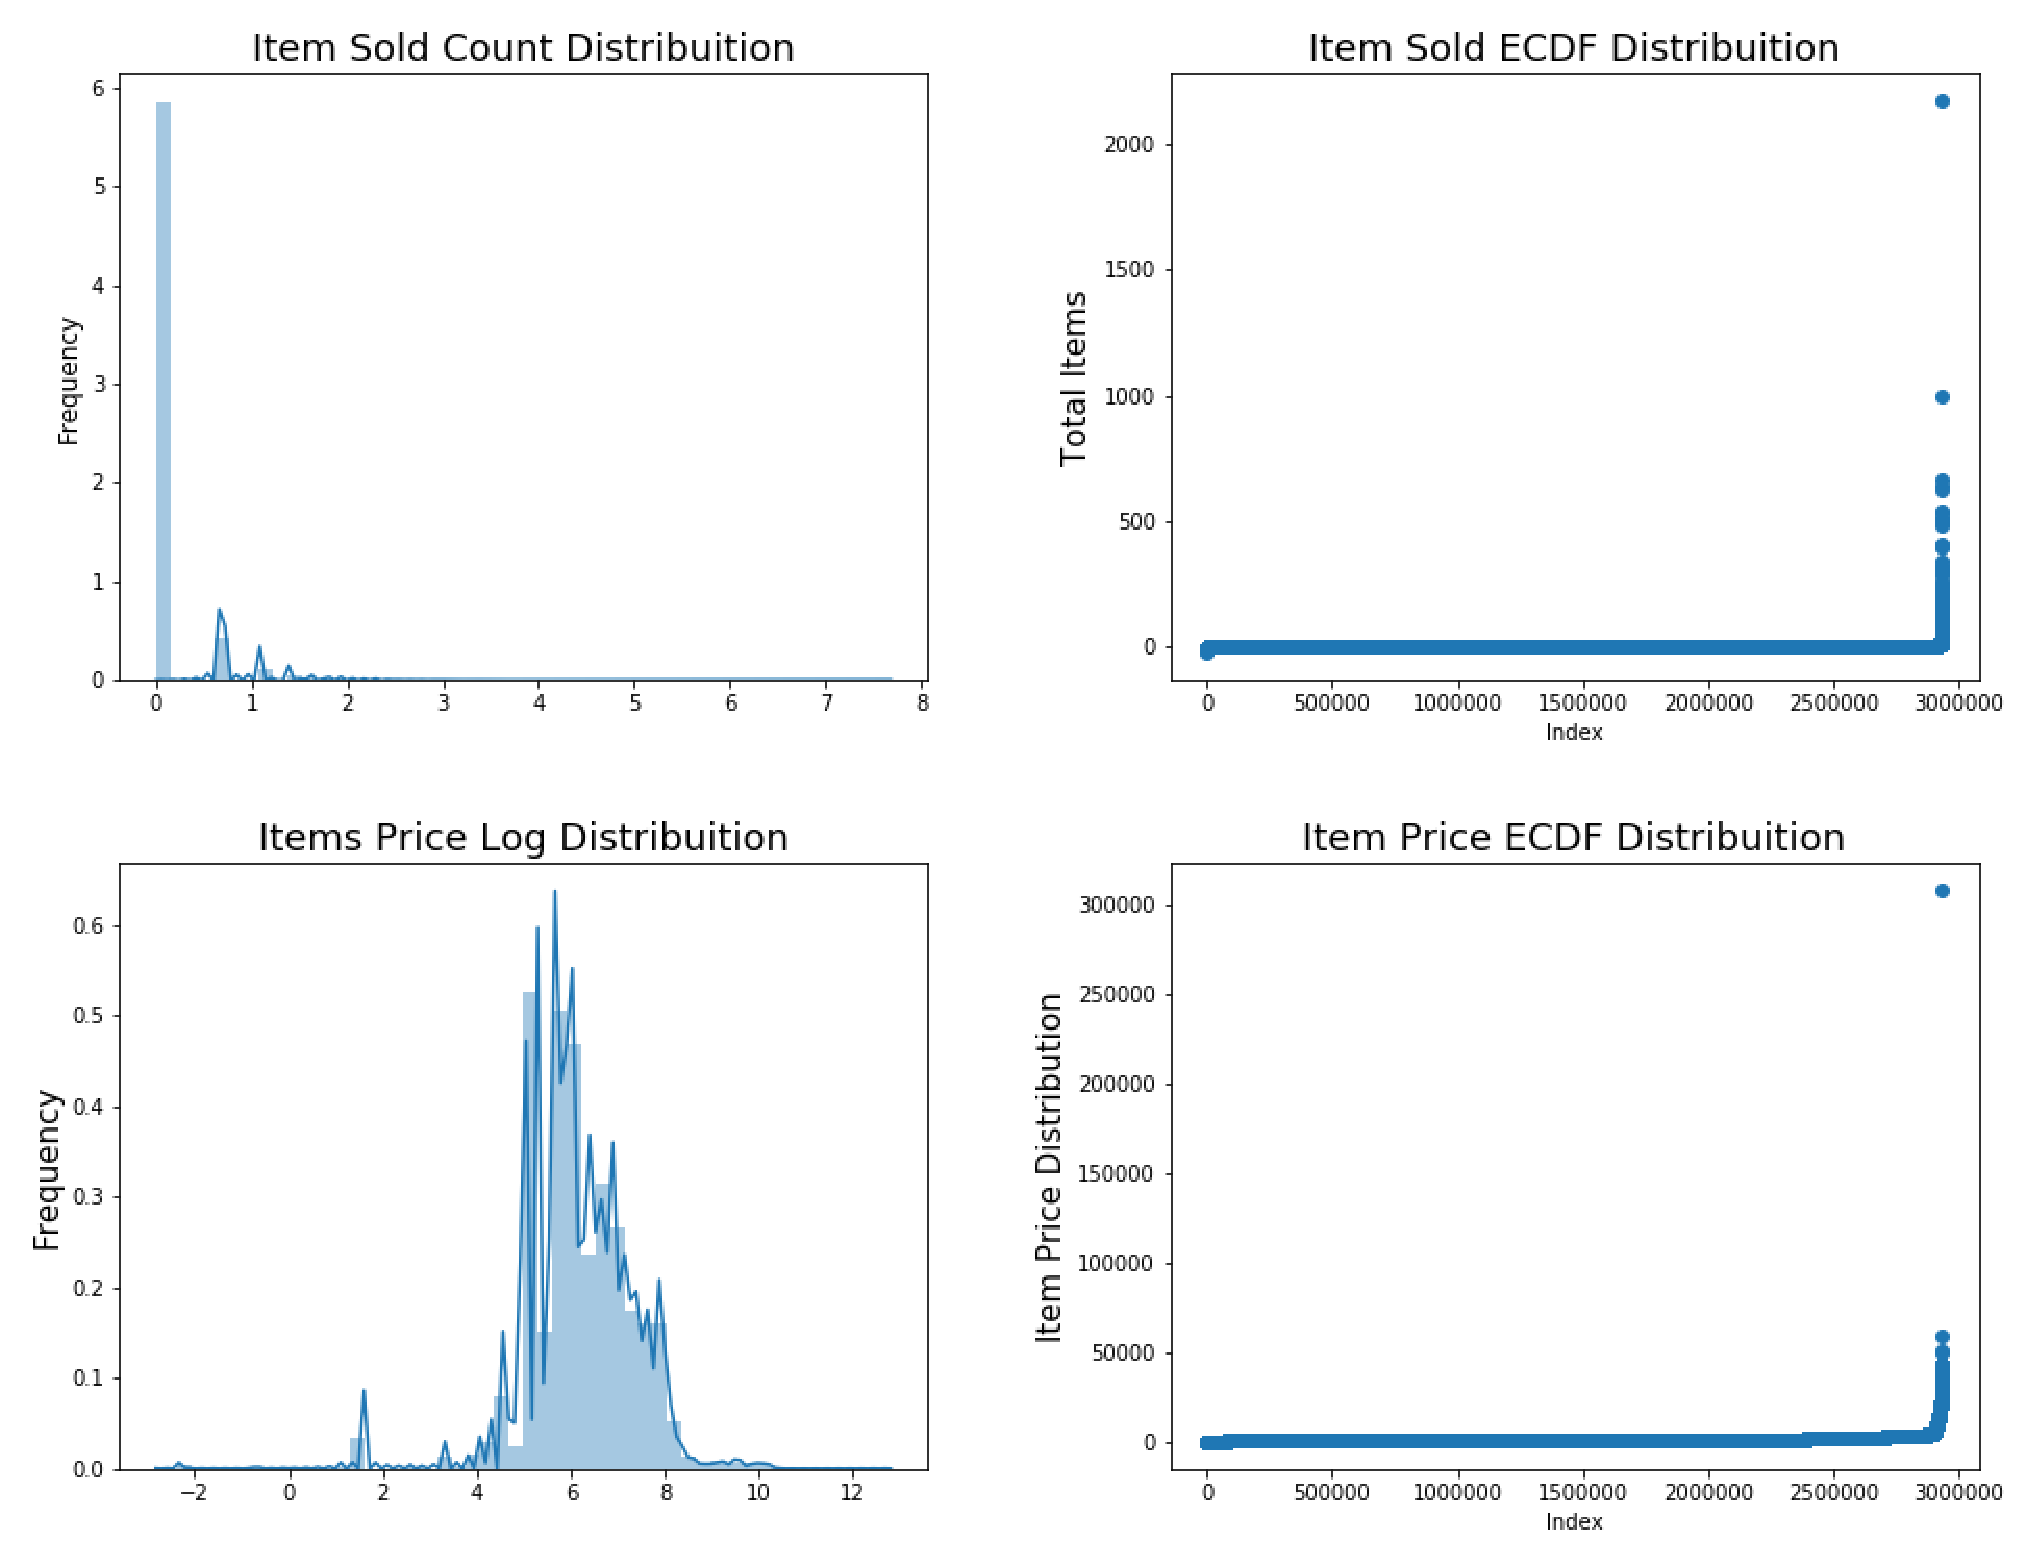
\includegraphics[width=.5\linewidth,height=.4\linewidth]{figures/scatterplot.eps}

	\end{center}
\end{slide}

\section{Feature Engineering}


\begin{slide}{Features importance}

	We take all of these features
	to form a new train datad.

	\begin{center}
		\includegraphics[width=.5\linewidth]{figures/FEATURE.eps}
	\end{center}

\end{slide}

\section{Methods}

\begin{slide}{Ensembling}

	To combine the 1st level model predictions,
	I'll use a simple linear regression.
	As I'm only feeding the model with
	predictions I don't need a complex model.

	\begin{center}
		\begin{itemize}
			\item Base Models
			      \
			      \begin{itemize}
				      \item RandomForest
				      \item XGBoost
				      \item LSTM
				      \item Linear regression
				      \item KNN
			      \end{itemize}
			\item Ensemble Model
			      \
			      \begin{itemize}
				      \item Linear regression
			      \end{itemize}
		\end{itemize}
	\end{center}
\end{slide}

\begin{slide}{Route}

	Here is an image to help the understanding

	\begin{center}
		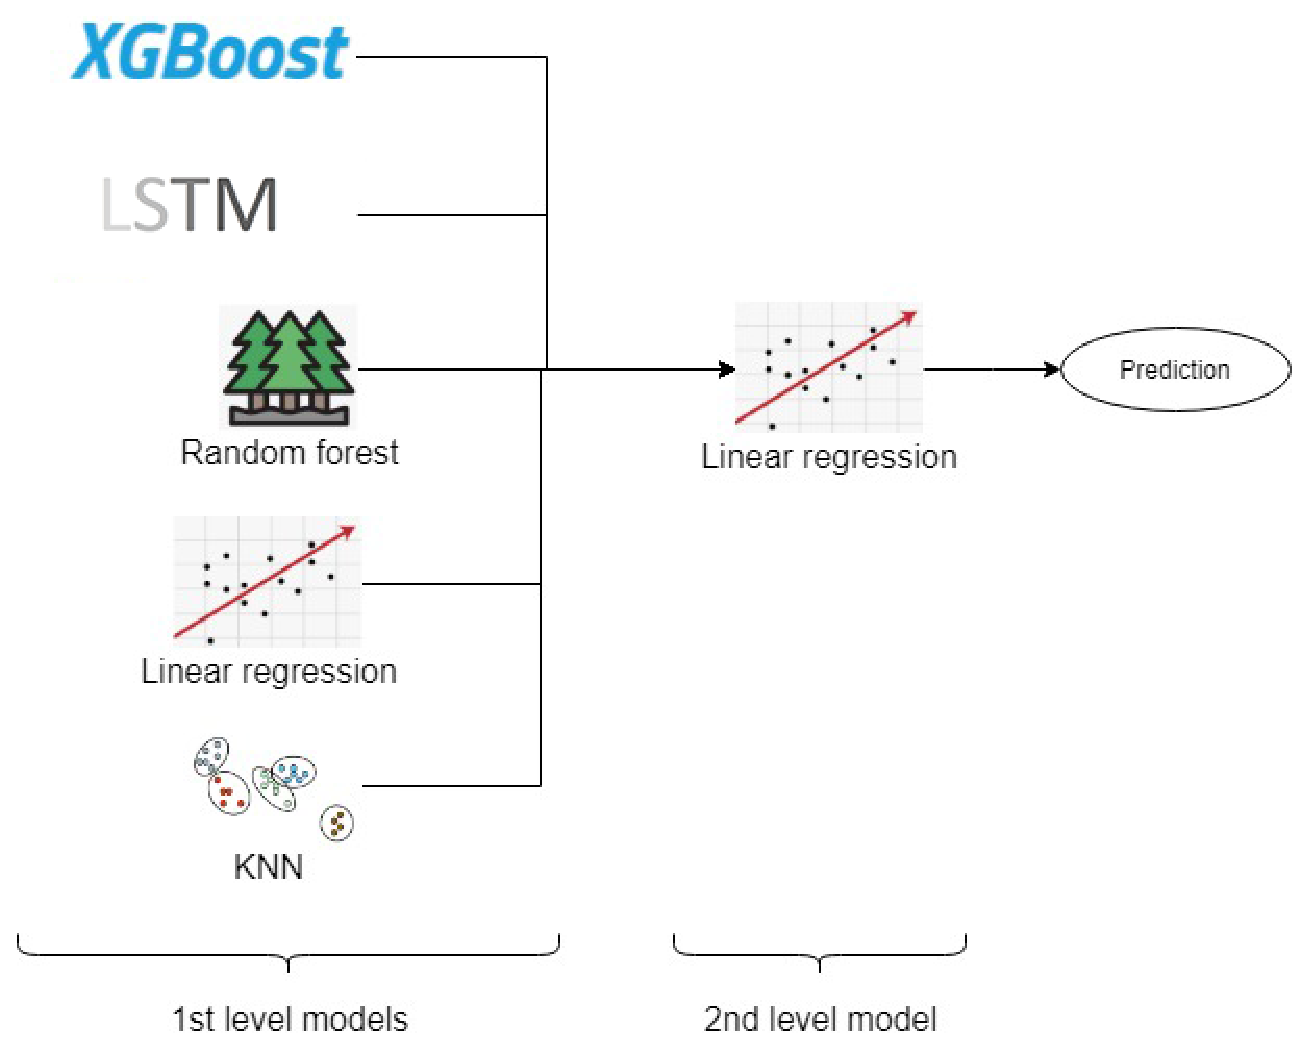
\includegraphics[width=.5\linewidth]{figures/Ensemble.eps}
	\end{center}

\end{slide}

\section{Forecast Results}

\begin{slide}{Evaluation Methods}
	\begin{center}
		\begin{itemize}
			\item RMSE
		\end{itemize}
	\end{center}

\end{slide}
%%==========================================================================================
%%
\begin{slide}{Forecast Results}
	\begin{itemize}
		\item The following are the best Score in training of the base models.
	\end{itemize}
	\begin{center}
		\begin{table}[h]  \centering
			\caption{Best Score of the Base Models}
			\label{tbl:best_score_base_models_old}
			\begin{tabular}{ccccccc}
				%\bottomrule
				\toprule
				                & RandomForest & XGBoost & LSTM   & Linear regression & KNN
				\\
				\midrule
				Train rmse      & 0.8358       & 0.8327  & 0.9276 &
				0.8572          & 0.6976                                                    \\
				Validation rmse & 0.8810       & 0.8959  & 0.6611 &
				0.8806          & 0.8946                                                    \\
				\bottomrule
			\end{tabular}
		\end{table}
	\end{center}
	\begin{itemize}
		\item Ensemble model means using
		      more than 1 model to finish the prediction.
		      The train rmse is 0.764973649571408.
	\end{itemize}

\end{slide}
%%
%%==========================================================================================


%%
%%==========================================================================================


\section{Conclusion}

%%==========================================================================================
%%
\begin{slide}[toc=,bm=]{Conclusion}
	\begin{description}
		\item Exploratory data analysis is
		      very important for the competition,
		      Discover the imperfections of the
		      data and have a certain understanding
		      of the overall appearance of the data,
		      which will help later modeling and analysis.
		\item The data that we have,
		      needed processed in many cases.
		      Data preprocessing includes
		      deal with missing data and outliers,
		      We must think carefully about the outliers,
		      such as ignoring them.
		\item The most important thing is
		      feature engineering.
		      We have to think carefully and
		      deal with outliers, such as ignoring
		      or deleting them.
		\item There is no best model,
		      only the best model. We should
		      try as many models as possible to
		      get the best prediction results.
		\item Feature engineering is very
		      important and even plays a decisive
		      role in this competition.
		\item The Ensemble model may perform better
		      than a single model when dealing
		      with some complex problems.
	\end{description}



\end{slide}

\begin{wideslide}[toc=,bm=]{}
	\centering
	\vspace{\stretch{1}}
	\twocolumn[
		lcolwidth=0.35\linewidth,
		rcolwidth=0.65\linewidth
	]
	{
		% \centerline{\includegraphics[scale=.2]{tulip-logo.eps}}
	}
	{
		\vspace{\stretch{1}}


		\textcolor{black}{\scalebox{2.0}{Thank you \& Question}}


	}
	\vspace{\stretch{1}}
\end{wideslide}

\end{document}
\endinput
